\ifgerman{\chapter{Implementation}}{\chapter{Implementation}}
\label{ch:implementation}

This chapter describes in detail how data is collected, what preprocessing techniques are applied to the data in order to make it fit for the machine learning algorithm to learn, how data is resampled, how it is clustered and what are the details of the architecture of the models and what are the evaluation strategies applied. This chapter will also detail all the tools and libraries that are used for achieving the above-mentioned tasks.

\section{Data Collection}

To begin with the implementation, the first step is to obtain the data. Obtaining the data is particularly challenging as these summaries are frequently changing, so scraping the data at different times results in the different assignment of a single document in different categories. Also, another challenge is that when documents for English and German are scraped separately, it happened quite often that some of the documents from one of the language are missing. Due to these challenges, a carefully crafted scraper which scrapes the data only if the documents from both of the languages are available, this, in turn, added a time overhead.

For scraping the data, Python library \textit{urllib}\footnote{https://docs.python.org/3/library/urllib.html} is used, this library scraps the HTML data out of the desired web pages. Then Python library \textit{Beautiful Soup}\footnote{https://www.crummy.com/software/BeautifulSoup/bs4/doc/} is used on the data collected from the web pages to parse the HTML content and produce a simple text document. During the parsing of the data, the corresponding label of the document is also parsed in order to complete the training dataset. First, the title of the document is scraped. Then all the HTML elements of the web page are removed to construct the text document. A new folder with the name of the category that is the label of the document is then used to store the documents of that class, and each document is given the corresponding title as the name of the file.

The EUR-Lex data set is an imbalanced dataset. That is the number of instances across the classes is not even as shown in \ref{fig:dataimbalance}.

\begin{figure}[!ht]
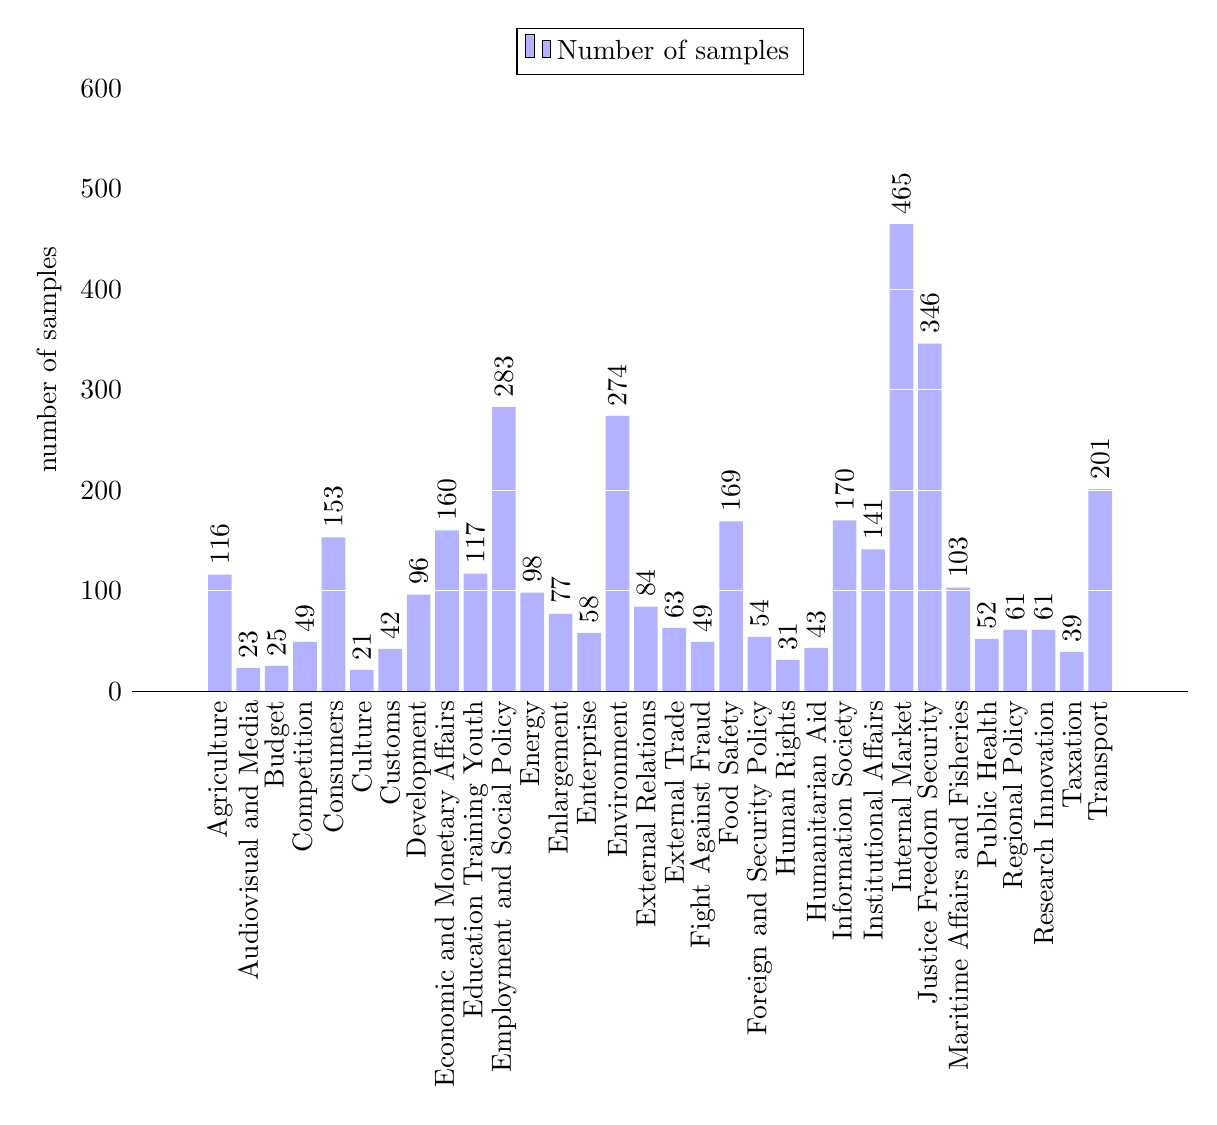
\begin{tikzpicture}
  \centering
  \begin{axis}[
        ybar, axis on top,
        %title={Cumulative Progress of Works},
        height=10cm, width=15cm,
        bar width=0.3cm,
        ymajorgrids, tick align=inside,
        major grid style={draw=white},
        enlarge y limits={value=.1,upper},
        x tick label style={rotate=90,anchor=east},
        ymin=0, ymax=600,
        axis x line*=bottom,
        axis y line*=left,
        y axis line style={opacity=0},
        tickwidth=0pt,
        enlarge x limits=true,
        legend style={
            at={(0.5,1)},
            anchor= north,
            legend columns=-1,
            /tikz/every even column/.append style={column sep=0.8cm}
        },
        ylabel={number of samples},
        symbolic x coords={
            Agriculture,
            Audiovisual and Media,
            Budget,
            Competition,
            Consumers,
            Culture,
            Customs,
            Development,
            Economic and Monetary Affairs,
            Education Training Youth,
            Employment and Social Policy,
            Energy,
            Enlargement,
            Enterprise,
            Environment,
            External Relations,
            External Trade,
            Fight Against Fraud,
            Food Safety,
            Foreign and Security Policy,
            Human Rights,
            Humanitarian Aid,
            Information Society,
            Institutional Affairs,
            Internal Market,
            Justice Freedom Security,
            Maritime Affairs and Fisheries,
            Public Health,
            Regional Policy,
            Research Innovation,
            Taxation,
            Transport},
       xtick=data,
       nodes near coords,        
       every node near coord/.append style={color=black,rotate=90, anchor=west }
       %x tick label style={rotate=90,anchor=east},
       %nodes near coords={
       % \pgfmathprintnumber[precision=0]{\pgfplotspointmeta}
        %}
    ]
    \addplot [draw=none, fill=blue!30] coordinates {
     (Agriculture,116)
(Audiovisual and Media, 23)
(Budget, 25)
(Competition, 49)
(Consumers, 153)
(Culture, 21)
(Customs, 42)
(Development, 96)
(Economic and Monetary Affairs, 160)
(Education Training Youth, 117)
(Employment and Social Policy, 283)
(Energy, 98)
(Enlargement, 77)
(Enterprise, 58)
(Environment, 274)
(External Relations, 84)
(External Trade, 63)
(Fight Against Fraud, 49)
(Food Safety, 169)
(Foreign and Security Policy, 54)
(Human Rights, 31)
(Humanitarian Aid, 43)
(Information Society, 170)
(Institutional Affairs, 141)
(Internal Market, 465)
(Justice Freedom Security, 346)
(Maritime Affairs and Fisheries, 103)
(Public Health, 52)
(Regional Policy, 61)
(Research Innovation, 61)
(Taxation, 39)
(Transport, 201) };
\legend{Number of samples}
  \end{axis}
  \end{tikzpicture}
      \captionsetup{justification=centering,margin=1cm}
      \caption{Document Distribution of EUR-Lex summaries}
    \label{fig:dataimbalance}
\end{figure}

\section{Data Cleaning}
The preprocessing involves removing of \textit{punctuation's}, \textit{numbers}, \textit{currency symbols} as they do not contribute anything in the classification process. Then the next step is to normalize the text, and this step is necessary because of the \textit{inflection} added due to the modification of words. Lemmatization is used here to normalize the text. As the last step, \textit{stop words} from both the languages are removed because, because they also do not contribute anything, and they increase the training time of the algorithm. For German language, \textit{umlauts - ä, ö and ü} are converted into its base form that is \textit{ä} to \textit{ae}, \textit{ö} to \textit{oe} and \textit{ü} to \textit{ue}. There were other Unicode characters which were also removed.

Following are the steps in which the preprocessing is done.

\begin{enumerate}
    \item As a first step, \textit{stop words} are removed.
    \item Next step is to lemmatize the words.
    \item Removal of other unnecessary symbols. For example, § is the symbol of a paragraph and is extensively used in the legal text. • is also another example.
    \item Removal of numbers
    \item Removal of punctuation 
    \item Conversion of umlauts to its base form.
\end{enumerate}

The order of the steps is also essential as it will help in reducing the overload on some of the processes. For example, when the stop words are removed in the first step, then the lemmatizer would not have to go through those words, and that will decrease the time taken to process the text. 

For removing the stop words Python library \textit{NLTK}\footnote{https://www.nltk.org/} (Natural Language Toolkit) is used. It provides stop words in both English and German language. To lemmatize the words \textit{spaCy}\footnote{https://spacy.io/} library is used for both the languages. To remove unnecessary symbols, custom functions are written. Number removal and conversion of umlauts were also done using custom functions.


\section{Clustering} \label{clustering}

To cluster the data using the K-means algorithm, first, the value of $k$ is obtained using Silhouette score (see \ref{silout})  and Elbow Analysis (see \ref{elbow}). 

Silhouette score and elbow analysis is computed using \textit{scikit-learn}\footnote{https://scikit-learn.org/stable/} library. First the documents from English corpus are converted into \gls{TF-IDF} vectors using the \textit{scikit-learn} library. These \gls{TF-IDF} vectors are then used for training $8$ k-means cluster which produces the cluster assignments for each value of $k$. The value 8 is heuristic as having more than 8 clusters would not be feasible in the context of the amount of resources than required for training the classifiers for these clusters and also, dividing data into more than 8 clusters would leave less data for classification in those clusters. The cluster assignments are then used along with the \gls{TF-IDF} matrix to find the silhouette score. The highest value of silhouette score means better the assignment of the clusters (see \ref{silout})

The values of silhoutte score obtained for EUR-Lex summaries are listed below in the \ref{table:silhoutteScore}
\begin{table}[!ht]
\centering
\begin{tabular}{cc}
\hline
$k$ & Silhoutte score \\ \hline
2 & 0.05693 \\
3 & 0.04417 \\
4 & 0.04749 \\
5 & 0.05515 \\
6 & 0.05480 \\
7 & 0.05647 \\
8 & 0.05537 \\ \hline
\end{tabular}
\captionsetup{justification=centering,margin=1cm}
\caption{Silhoutte scores for 8 values of $k$}
\label{table:silhoutteScore}
\end{table}

And the elbow analysis for the same is shown in the \ref{fig:elbowAT2}, which indicates that the data should be divided into 2 clusters. The silhouette score is high at 2 clusters, that means that other values of $k$ will not model the data better. 

\begin{figure}[!ht]
    \centering
    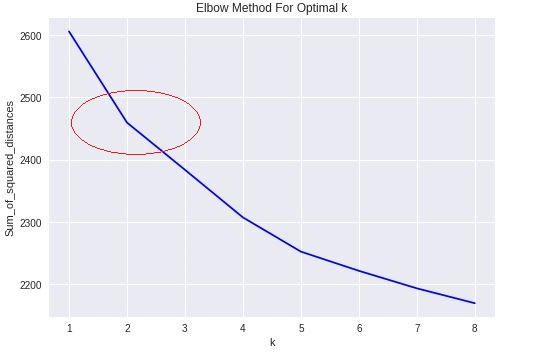
\includegraphics[width=8cm, height=5.5cm]{pics/ElbowAT2.jpg}
    \captionsetup{justification=centering,margin=1cm}
    \caption{Elbow analysis validating the value of $k$ at 2}
    \label{fig:elbowAT2}
\end{figure}

After obtaining the value of $k = 2$ for the number of clusters, the next step is to apply constrained k-means clustering, for this an open source implementation of constrained k-means is used here called as \textit{COP-Kmeans}\footnote{https://github.com/Behrouz-Babaki/COP-Kmeans} \cite{behrouz_babaki_2017_831850}. 

The COP-Kmenas requires the dataset (\gls{TF-IDF} matrix of the corpus), the value of $k$, and two lists of constraints (must-link and cannot-link). As mentioned already, no prior information is available for the cannot-link constraints; hence, only must-link constraints are applied. 

The \ref{table:ClusterAssignments32Classes} shows the cluster assignments of all the 32 categories of the EUR-Lex summaries obtained after applying COP-K-means with $k=2$.


\begin{table}[!ht]
\centering
\begin{tabular}{cc}
\hline
\textbf{Class Label} & \textbf{Cluster Assignment} \\ \hline
Agriculture & 1 \\ 
Audiovisual and Media & 1 \\ 
Budget & 2 \\ 
Competition & 1 \\ 
Consumers & 1 \\ 
Culture & 2 \\ 
Customs & 2 \\ 
Development & 2 \\ 
Economic and Monetary Affairs & 2 \\ 
Education Training Youth & 2 \\ 
Employment and Social Policy & 1 \\ 
Energy & 1 \\ 
Enlargement & 2 \\ 
Enterprise & 1 \\ 
Environment & 1 \\ 
External Relations & 2 \\ 
External Trade & 2 \\ 
Fight Against Fraud & 2 \\ 
Food Safety & 1 \\ 
Foreign and Security Policy & 2 \\ 
Human Rights & 2 \\ 
Humanitarian Aid & 2 \\ 
Information Society & 1 \\ 
Institutional Affairs & 2 \\ 
Internal Market & 1 \\ 
Justice Freedom Security & 2 \\ 
Maritime Affairs and Fisheries & 2 \\ 
Public Health & 1 \\ 
Regional Policy & 2 \\ 
Research Innovation & 2 \\ 
Taxation & 1 \\ 
Transport & 1 \\ \hline
\end{tabular}
\captionsetup{justification=centering,margin=1cm}
\caption{Assignment of EUR-Lex summaries into clusters}
\label{table:ClusterAssignments32Classes}
\end{table}
\clearpage
\section{Data Resampling} \label{dataResampling}
The method behind the resampling of the dataset is to loop over the dataset one by one to find duplicate documents. When a duplicate document is found, check the labels of all the duplicate documents and compare the total number of samples in all the labels for which the duplicate documents are found. Remove the duplicate instance from the class containing the most number of samples. This method is time consuming as the number of loops the algorithm goes through before finishing is $n$ x $n$ where $n$ is the number of documents.

To make the algorithm more efficient, first, the total number of samples are counted. Then, a list of non-duplicate documents without the labels is created. The generated list is then used to iterate over all the duplicate documents, by comparing every document and storing the corresponding labels of the duplicate document. After a single document from the non duplicated list completes iterating over all the duplicate documents, the labels of the duplicated documents are checked for its class distribution, and then the duplicated document is removed from the majority class. Also, if a duplicate document is found in the same class, then only one is kept, and the other is removed.

The pseudo code for the above-mentioned algorithm where $x$ is a list of non duplicated documents. $x_{d}$ is the list with duplicated documents and $y_{d}$ contains the corresponding labels for the $x_{d}$. 

\begin{algorithm}
\caption{Resampling Algorithm}
\begin{algorithmic}[1]
\FOR {all label $\mathscr{L}$ in $y_{d}$}
    \STATE $\text{dist} \leftarrow \text{Counter}(\mathscr{L})$
\ENDFOR

\FOR{$i = 1:\text{count}(x)$}
    \STATE $x_{i} \leftarrow x[i]$
    \FOR{$j = 1:\text{count}(x_{d}, y_{d})$}
        \STATE $x_{j} \leftarrow x_{d}[j]$
        \STATE $y_{j} \leftarrow y_{d}[j]$
        \IF{$x_{i} == x_{j}$}
            \STATE $\text{tmp\_list} \leftarrow y_{j}$ 
         \ENDIF
    \ENDFOR
    \IF {$len(\text{tmp\_list}) == 1$}
        \STATE $\ell \leftarrow tmp\_list$
    \ELSE
        \FOR {$k =1:\text{count}(\text{tmp\_list})$}
            \STATE $\ell \leftarrow min(\text{dist}[\text{temp\_list}[k]])$
        \ENDFOR
    \ENDIF
    \STATE $x_{i} \rightarrow doc$    \COMMENT{Resampled document data}
    \STATE $\ell \rightarrow \textit{labels}$ \COMMENT{Labels for the resampled document data}
\ENDFOR
\end{algorithmic}
\end{algorithm}

\ref{table:befforeAfterResampling} shows the total number of documents in the original dataset and the number of documents after the resampling technique is applied.

\begin{table}[!ht]
\centering
\begin{tabular}{lcc}
\hline
\multicolumn{1}{c}{Category} & Original & Resampled \\ \hline
Agriculture & 116 & 90 \\
Audiovisual and Media & 23 & 18 \\
Budget & 25 & 25 \\
Competition & 49 & 47 \\
Consumers & 153 & 125 \\
Culture & 21 & 21 \\
Customs & 42 & 39 \\
Development & 96 & 63 \\
Economic and Monetary Affairs & 160 & 149 \\
Education Training Youth & 117 & 102 \\
Employment and Social Policy & 283 & 174 \\
Energy & 98 & 74 \\
Enlargement & 77 & 64 \\
Enterprise & 58 & 56 \\
Environment & 274 & 134 \\
External Relations & 84 & 59 \\
External Trade & 63 & 56 \\
Fight Against Fraud & 49 & 31 \\
Food Safety & 169 & 108 \\
Foreign and Security Policy & 54 & 49 \\
Human Rights & 31 & 35 \\
Humanitarian Aid & 43 & 30 \\
Information Society & 170 & 149 \\
Institutional Affairs & 141 & 128 \\
Internal Market & 465 & 234 \\
Justice Freedom Security & 346 & 223 \\
Maritime Affairs and Fisheries & 103 & 90 \\
Public Health & 52 & 52 \\
Regional Policy & 61 & 58 \\
Research Innovation & 61 & 55 \\
Taxation & 39 & 39 \\
Transport & 201 & 139 \\ \cline{1-3}
\end{tabular}
\captionsetup{justification=centering,margin=1cm}
\caption{Distribution of number of samples before and after resampling}
\label{table:befforeAfterResampling}
\end{table}
\section{Training the Word Vectors}

The model used in the creation of the word vectors is a neural network, and neural networks are data hungry as it requires a lot of data to train them properly. As a result, another domain-specific dataset is used in this experiment because dataset used for classification is small. Hence, the whole EUR-Lex dataset was used as it contains 19,348 documents mostly consisting regulations, decisions and directives of European Union \cite{jf:SemanticLaw}.

\subsection{Training Cross Lingual Word Embedding}\label{implementationCrossLingual}

I am using the technique suggested by Duong et. al \cite{duong-EtAl:2016:EMNLP} (see \ref{backgroundCrosslingual}) to train bilingual domain-specific word embeddings.
The dataset used for training the domain-specific word embeddings is the EUR-Lex dataset, as the dataset used for classification (EUR-Lex summaries) is less compared to the EUR Lex dataset. For creating a bilingual dictionary, \textit{EuroVoc} thesaurus \cite{steinberger2002cross} provided by Publication office of the European Union will be used. It is available in 24 official languages recognized by the European Union. This thesaurus is domain-specific hence it does not involve common words that might occur in the documents. Due to this reason, this thesaurus is combined with bilingual dictionaries that are available from \textit{Facebook MUSE} \cite{conneau2017word}. These bilingual dictionaries were created using Facebook's internal translation tools. The authors claim that these dictionaries handle the polysemy of the words better. This combined bilingual dictionary with the original EUR-Lex dataset is used to create the legal domain-specific bilingual word embeddings. 

Monolingual word embeddings for training \gls{BiLSTM} is trained using \textit{Skip-gram} method with Fasttext\footnote{https://fasttext.cc/docs/en/cr awl-vectors.html}\cite{graves2009novel} tool. These embeddings were also trained on EUR-Lex corpus. These monolingual word embeddings are in English and German language and are in 300 dimensions.

For training general-purpose bilingual word embedding we will be again using Fasttext which provides word embeddings in 157 languages on Wikipedia\footnote{https://www.wikipedia.org/} and Common Crawl\footnote{http://commoncrawl.org/} data and is trained using Continuous bag-of-words model in dimension 300. The word embeddings for multiple languages cannot be combined together because they belong in different vector space. Facebook's MUSE\footnote{https://github.com/facebookresearch/MUSE} \cite{conneau2017word} with the help of parallel dictionaries are used to align both word embeddings (English and German) into a single vector space. Upon alignment, both the embeddings can be simply concatenated and can be used for classification purpose. These word embeddings are created from various sources, it contains text from various domains and hence it will hence they are being used as general-purpose word embeddings.

\section{Architecture and Training}
This section describes in detail the specifics of architectures of the algorithm used for all the three questions mentioned in \ref{sec:conceptRQ}.

Before beginning to train the models, it is necessary to divide the dataset into a training set and a testing set. Generally, 70\% of the data is for training purposes, and 30\% to evaluate the model. This division is stratified, which means that the class distribution in training and testing set will remain almost equal. The stratified division ensures that there are enough examples for each class in training, and test phase of the model. 

Neural network based classification models are prone to \textit{overfitting} \cite{Prechelt1998}. Overfitted model will perform well on the training data but fail to perform well on the testing data. To put it simply, while training the error on the training set will keep on decreasing and the error on the unseen data starts getting worst. To avoid this situation regularization techniques such as Dropout, L1 and L2 regularization and early stopping are used.

Dropout and L1, L2 regularization are explicit regularization technique, that is it explicitly reduces the model complexity. In Dropout regularization techniques, during the training, a fraction of randomly selected neurons are ignored. Hence, their activation contribution to the forward pass and weight updates are removed. While Dropout regularization reduces the model complexity by removing randomly selected neuron during training, L1 and L2 regularization reduce the model complexity by imposing a penalty to the weight of all the features and features with non zero weights respectively.      

On the other hand, early stopping regularization is implicit which does not affect the complexity of the model directly \cite{zhang2016understanding}. Early stopping, monitors the training process and halts it once the performance of the model starts degrading. It does so by monitoring the performance of the classifier on the validation data. 

Dropout, L2 regularization, and early stopping can be configured in \textit{keras} while building the model. During the training, we split 30\% of training data for validation purpose so that there is no need for splitting validation data at the time when we split the dataset into training and testing set.

\subsection{First Research Question} \label{impQuestion1}

In the first research question \gls{SVM} are compared to \glspl{BiLSTM}. When using an \gls{SVM} algorithm, we do not know beforehand the value of $C$. To find that out, we need some kind of selection mechanism. The aim is to find out the value of $C$ such that it can predict accurately on unknown data. One method of finding the value of $C$ is called \textit{Grid Search Cross Validation} (Grid Search CV). This method is straight forward; first, we select the number of values of $C$, then we divide the training set into $n$ equal-sized subsets. Then we train the \gls{SVM} using one value from $C$ on the $n-1$ subset and predict on the one left subset, we repeat this process until every instance of the training set is predicted once for every value of $C$.

This process is computationally expensive as each subset will be trained on every value of $C$. We used the following values of $C$ (0.001,0.01, 0.1,1,10,100).

To train \gls{SVM}, \gls{TF-IDF} matrix of the English corpus is created using the \textit{scikit-learn} python library and then this \gls{TF-IDF} matrix is used to train a linear \gls{SVM} from the same \textit{scikit-learn} library. 

The \gls{SVM} is compared against two \gls{BiLSTM} models, one without clustered data on single language (English) and one with clustered data (English and German). The technique used for training both \gls{SVM} and \gls{BiLSTM} is different, while \gls{SVM} is trained on whole documents, \glspl{BiLSTM} are trained on sentences created using sliding window technique (see \ref{backgroundSlidingWindow}, \ref{question1}). The \ref{fig:PlainLSTM} shows the architecture of the \gls{BiLSTM} model trained on English corpus with all the 32 classes. The \gls{BiLSTM} models were created using \textit{Keras}\footnote{https://keras.io/} python library. 

The hyperparameter for \gls{BiLSTM} trained on English corpus without clustered data is listed in \ref{table:hyperparameterLSTM32class}. 

\begin{table}[!ht]
\centering
\begin{tabular}{cc}
\hline
\textbf{Hyperparameter} & \textbf{Value} \\ \hline
Sentence Size & 30 words \\
Batch Size & 32 \\
Embedding Dimension & 200 \\
Hidden 1 Size & 40 \\
Hidden 2 Size & 40 \\
Dropout 1 & 0.5 \\
Dropout 2 & 0.5 \\
$l2$ regularization 1 & 0.04 \\
$l2$ regularization 2 & 0.01 \\
Learning Rate & 0.001 \\ \hline
\end{tabular}
 \captionsetup{justification=centering,margin=1cm}
\caption{Hyperparameter of \gls{BiLSTM} for training English language corpus without clustered data}
\label{table:hyperparameterLSTM32class}
\end{table}


\begin{figure}[!ht]
    \centering
    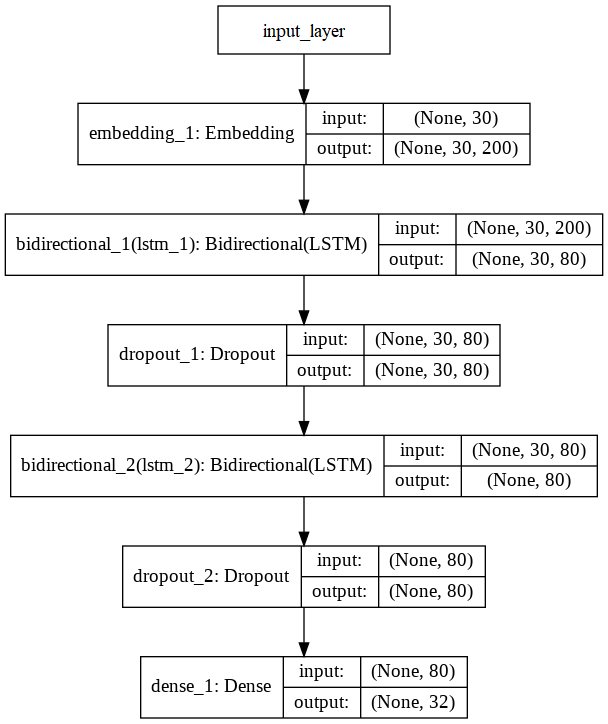
\includegraphics[width=9cm, height=11cm]{pics/EN_32.png}
    \captionsetup{justification=centering,margin=1cm}
    \caption{Architecture of \gls{BiLSTM} for training English language corpus without clustered data}
    \label{fig:PlainLSTM}
\end{figure}
\clearpage
The hyperparameter for the \glspl{BiLSTM} used on clustered data is exactly similar to the one without clustered data trained on English language \ref{table:hyperparameterLSTM32class}.

The architecture for \gls{BiLSTM} trained on cluster 1 and cluster 2 data is shown in \ref{fig:cluster1&2LSTM}.

\begin{figure}[!ht]
    \centering
    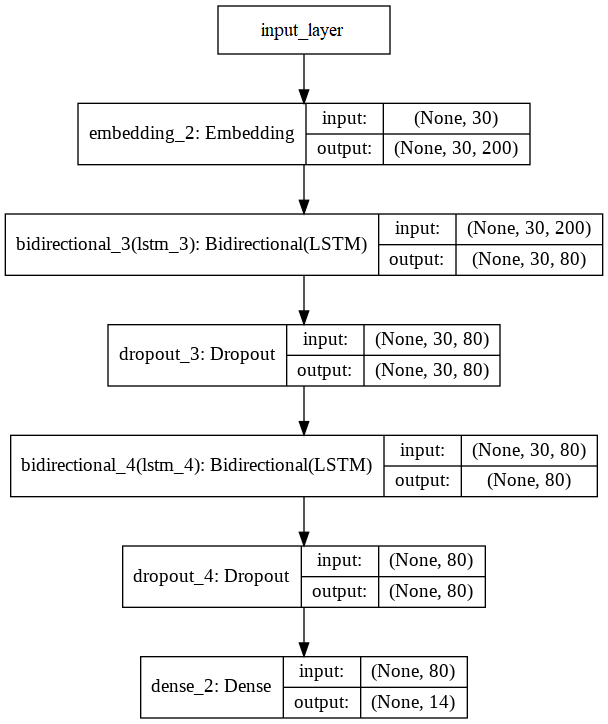
\includegraphics[width=9cm, height=12cm]{pics/LSTM_LEGALEMB_CLUSTER_1.png}
    \captionsetup{justification=centering,margin=1cm}
    \caption{Architecture of \gls{BiLSTM} for training English and German language corpus on cluster 1 and cluster 2 data}
    \label{fig:cluster1&2LSTM}
\end{figure}


\clearpage

\subsection{Second Research Question}
In the second question general-purpose embeddings is compared to word embeddings created using EUR-Lex corpus (see \ref{implementationCrossLingual}).

Both the approaches using the general-purpose resource and the domain-specific resources, uses \glspl{BiLSTM} trained on clustered data, similar to the \glspl{BiLSTM} in \ref{impQuestion1}
The hyperparameters for the both approaches is listed in \ref{table:FBMuseGeneralpurpose} for general-purpose embeddings and \ref{table:DomainSpecificHyperparameter} for domain-specific embeddings.

\begin{table}[!ht]
\centering
\begin{tabular}{cc}
\hline
\textbf{Hyperparameter} & \textbf{Value} \\ \hline
Sentence Size & 30 words \\
Batch Size & 32 \\
Embedding Dimension & 300 \\
Hidden 1 Size & 40 \\
Hidden 2 Size & 40 \\
Dropout 1 & 0.5 \\
Dropout 2 & 0.5 \\
$l2$ regularization 1 & 0.04 \\
$l2$ regularization 2 & 0.01 \\
Learning Rate & 0.001 \\ \hline
\end{tabular}
\captionsetup{justification=centering,margin=1cm}
\caption{Hyperparameter of \gls{BiLSTM} for training on English and German language with clustered data using general-purpose word embedding created using Facebook's MUSE python library}
\label{table:FBMuseGeneralpurpose}
\end{table}

\begin{table}[!ht]
\centering
\begin{tabular}{cc}
\hline
\textbf{Hyperparameter} & \textbf{Value} \\ \hline
Sentence Size & 30 words \\
Batch Size & 32 \\
Embedding Dimension & 200 \\
Hidden 1 Size & 40 \\
Hidden 2 Size & 40 \\
Dropout 1 & 0.5 \\
Dropout 2 & 0.5 \\
$l2$ regularization 1 & 0.04 \\
$l2$ regularization 2 & 0.01 \\
Learning Rate & 0.001 \\ \hline
\end{tabular}
\captionsetup{justification=centering,margin=1cm}
\caption{Hyperparameter of \gls{BiLSTM} for training on English and German language with clustered data using domain-specific word embedding created from EUR-Lex dataset}
\label{table:DomainSpecificHyperparameter}
\end{table}

The only difference between the training parameters of both the approaches is the embedding dimensions; the general-purpose embedding is in 300 dimensions whereas the domain-specific embedding is in 200 dimensions. The reason for this difference is that aligning two embeddings in a single vector space is a computationally inexpensive task, then learning the embedding from scratch for two languages. Decreasing the dimensions will result in the reduction of training time, and hence the dimension of domain-specific word embeddings are 100 less than general-purpose embeddings.

The architecture for \gls{BiLSTM} trained using general-purpose word embeddings is shown in \ref{fig:FBMuseCluster} and \gls{BiLSTM} trained using domain-specific word embeddings is show in \ref{fig:LegalEmbCluster}.

\begin{figure}[!ht]
    \centering
    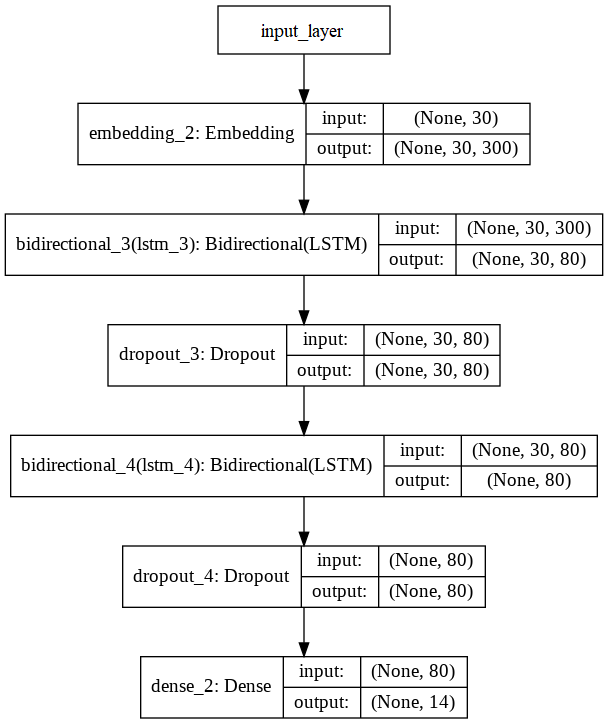
\includegraphics[width=9cm, height=12cm]{pics/FBMUSE_Untrained_cluster_1.png}
    \captionsetup{justification=centering,margin=1cm}
    \caption{Architecture of \gls{BiLSTM} for training English and German language corpus on cluster 1 and cluster 2 data using general-purpose embeddings created using Facebook MUSE python library}
    \label{fig:FBMuseCluster}
\end{figure}



\begin{figure}[!ht]
    \centering
    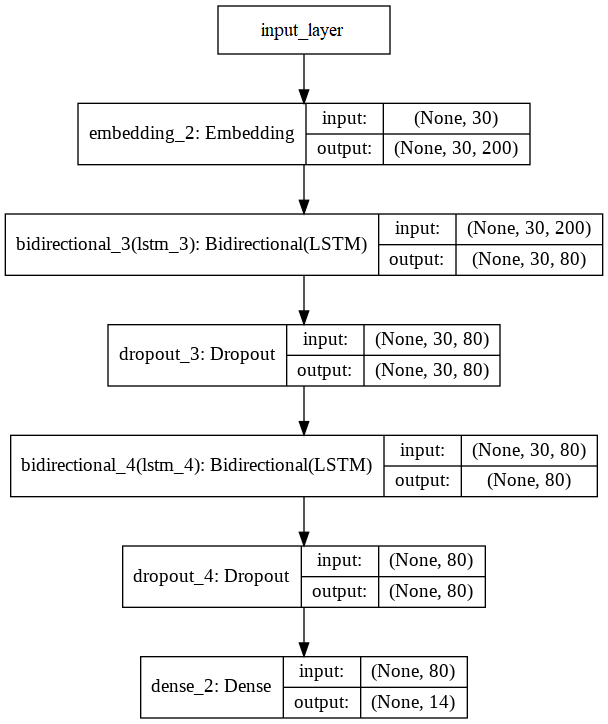
\includegraphics[width=9cm, height=12cm]{pics/LSTM_LEGALEMB_CLUSTER_1.png}
    \captionsetup{justification=centering,margin=1cm}
    \caption{Architecture of \gls{BiLSTM} for training English and German language corpus on cluster 1 and and cluster 2 data using general-purpose embeddings trained on EUR-Lex dataset}
    \label{fig:LegalEmbCluster}
\end{figure}

For evaluating the predictions, each document is divided into sentences using the same sliding window technique used to create the training data, then predictions are stored for every sentence of a document, and the predictions are summed up, and the class with the highest value is considered the class of the document. 

\subsection{Third Research Question}
The third question evaluates the capability of training multiple languages in a single \gls{BiLSTM} model compared to training different models for different languages. For this purpose two models, one for the English and another for the German language will be compared to a single model trained on both the English and the German language together.

Training on the clustering data will only be performed in the case where both the languages are used in a single model; this is due to the fact that performing clustering on a single language will reduce the number of samples in each cluster significantly. So for this question, one model with both the languages will be trained without clustering and one with clustering. 

The hyperparameters and architecture for all the models will be the same to ensure a fair comparison. The hyperparameters are for this question is listed in \ref{table:hyperParameterQuestion3} and the architecture for this question is shown in \ref{fig:architectureQuestion3}

\begin{table}[!ht]
\centering
\begin{tabular}{cc}
\hline
\textbf{Hyperparameter} & \textbf{Value} \\ \hline
Sentence Size & 30 words \\
Batch Size & 32 \\
Embedding Dimension & 300 \\
Hidden 1 Size & 40 \\
Hidden 2 Size & 40 \\
Dropout 1 & 0.5 \\
Dropout 2 & 0.5 \\
$l2$ regularization 1 & 0.04 \\
$l2$ regularization 2 & 0.03 \\
Learning Rate & 0.001 \\ \hline
\end{tabular}
\captionsetup{justification=centering,margin=1cm}
\caption{Hyperparameters of \gls{BiLSTM} for training on the English and the German language with and without clustered data and trained on both languages separately}
\label{table:hyperParameterQuestion3}
\end{table}

\begin{figure}[!ht]
    \centering
    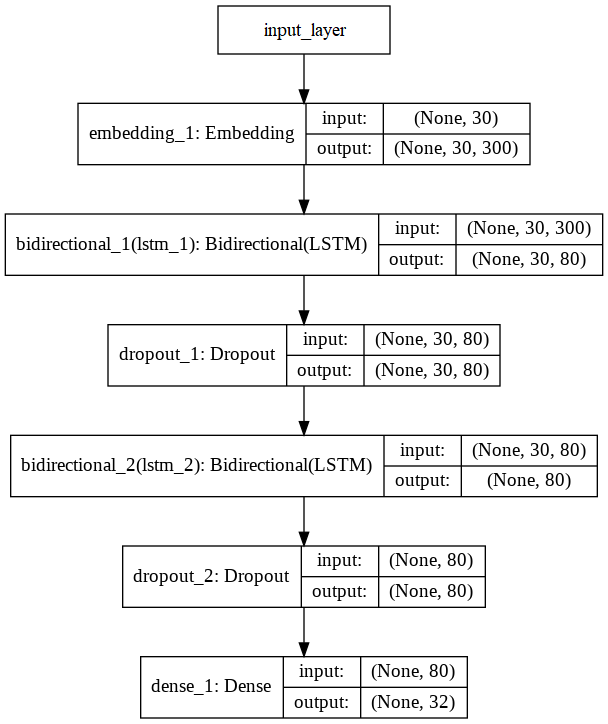
\includegraphics[width=9cm, height=12cm]{pics/Question3.png}
    \captionsetup{justification=centering,margin=1cm}
    \caption{Architecture of \gls{BiLSTM} for training on the English and the German language with and without clustered data and trained on both languages separately}
    \label{fig:architectureQuestion3}
\end{figure}

